%-------------------------
% Resume in Latex
% Author : Jake Gutierrez
% Based off of: https://github.com/sb2nov/resume
% License : MIT
%------------------------

\documentclass[letterpaper,11pt]{article}
\usepackage{geometry}
\usepackage{latexsym}
\usepackage[empty]{fullpage}
\usepackage{titlesec}
\usepackage{marvosym}
\usepackage[usenames,dvipsnames]{color}
\usepackage{verbatim}
\usepackage{enumitem}
\usepackage[hidelinks]{hyperref}
\usepackage{fancyhdr}
\usepackage[english]{babel}
\usepackage{tabularx}
\usepackage{float}
\usepackage{multicol}
\usepackage{xcolor}
\input{glyphtounicode}
\usepackage{hyperref}
\usepackage{lipsum}
\usepackage{graphicx}
\graphicspath{ {./} }
\hypersetup{
    colorlinks=true,
    linkcolor=blue,
    filecolor=magenta,      
    urlcolor=blue,
    pdfpagemode=FullScreen,
    }

\geometry{paperheight=2in, paperwidth=8.5in, left=0.3in, right=0.3in, top=0in, bottom=0in}
\setlength{\voffset}{-0.25in}
\setlength{\headsep}{5pt}

\linespread{1.1} 
%----------FONT OPTIONS----------
% sans-serif
% \usepackage[sfdefault]{FiraSans}
% \usepackage[sfdefault]{roboto}
% \usepackage[sfdefault]{noto-sans}
% \usepackage[default]{sourcesanspro}

% serif
% \usepackage{CormorantGaramond}
% \usepackage{charter}

%-------------------------
% Custom commands

%-------------------------------------------
%%%%%%  RESUME STARTS HERE  %%%%%%%%%%%%%%%%%%%%%%%%%%%%
\begin{document}
\write18{wget https://github.com/thienlongtran/resume-update-overleaf-sync/blob/main/gha-logo.png?raw=true}
\vspace*{\fill}

\begin{minipage}{0.6\textwidth}

Last Updated On: \underline{\today}\newline

This resume was updated using continuous integration through a GitHub Actions Workflow and Overleaf Git Sync. Check it out here:

\href{https://github.com/thienlongtran/resume-update-overleaf-sync}{https://github.com/thienlongtran/resume-update-overleaf-sync}
\end{minipage}
\hfill%
\begin{minipage}{0.3\textwidth}\raggedleft
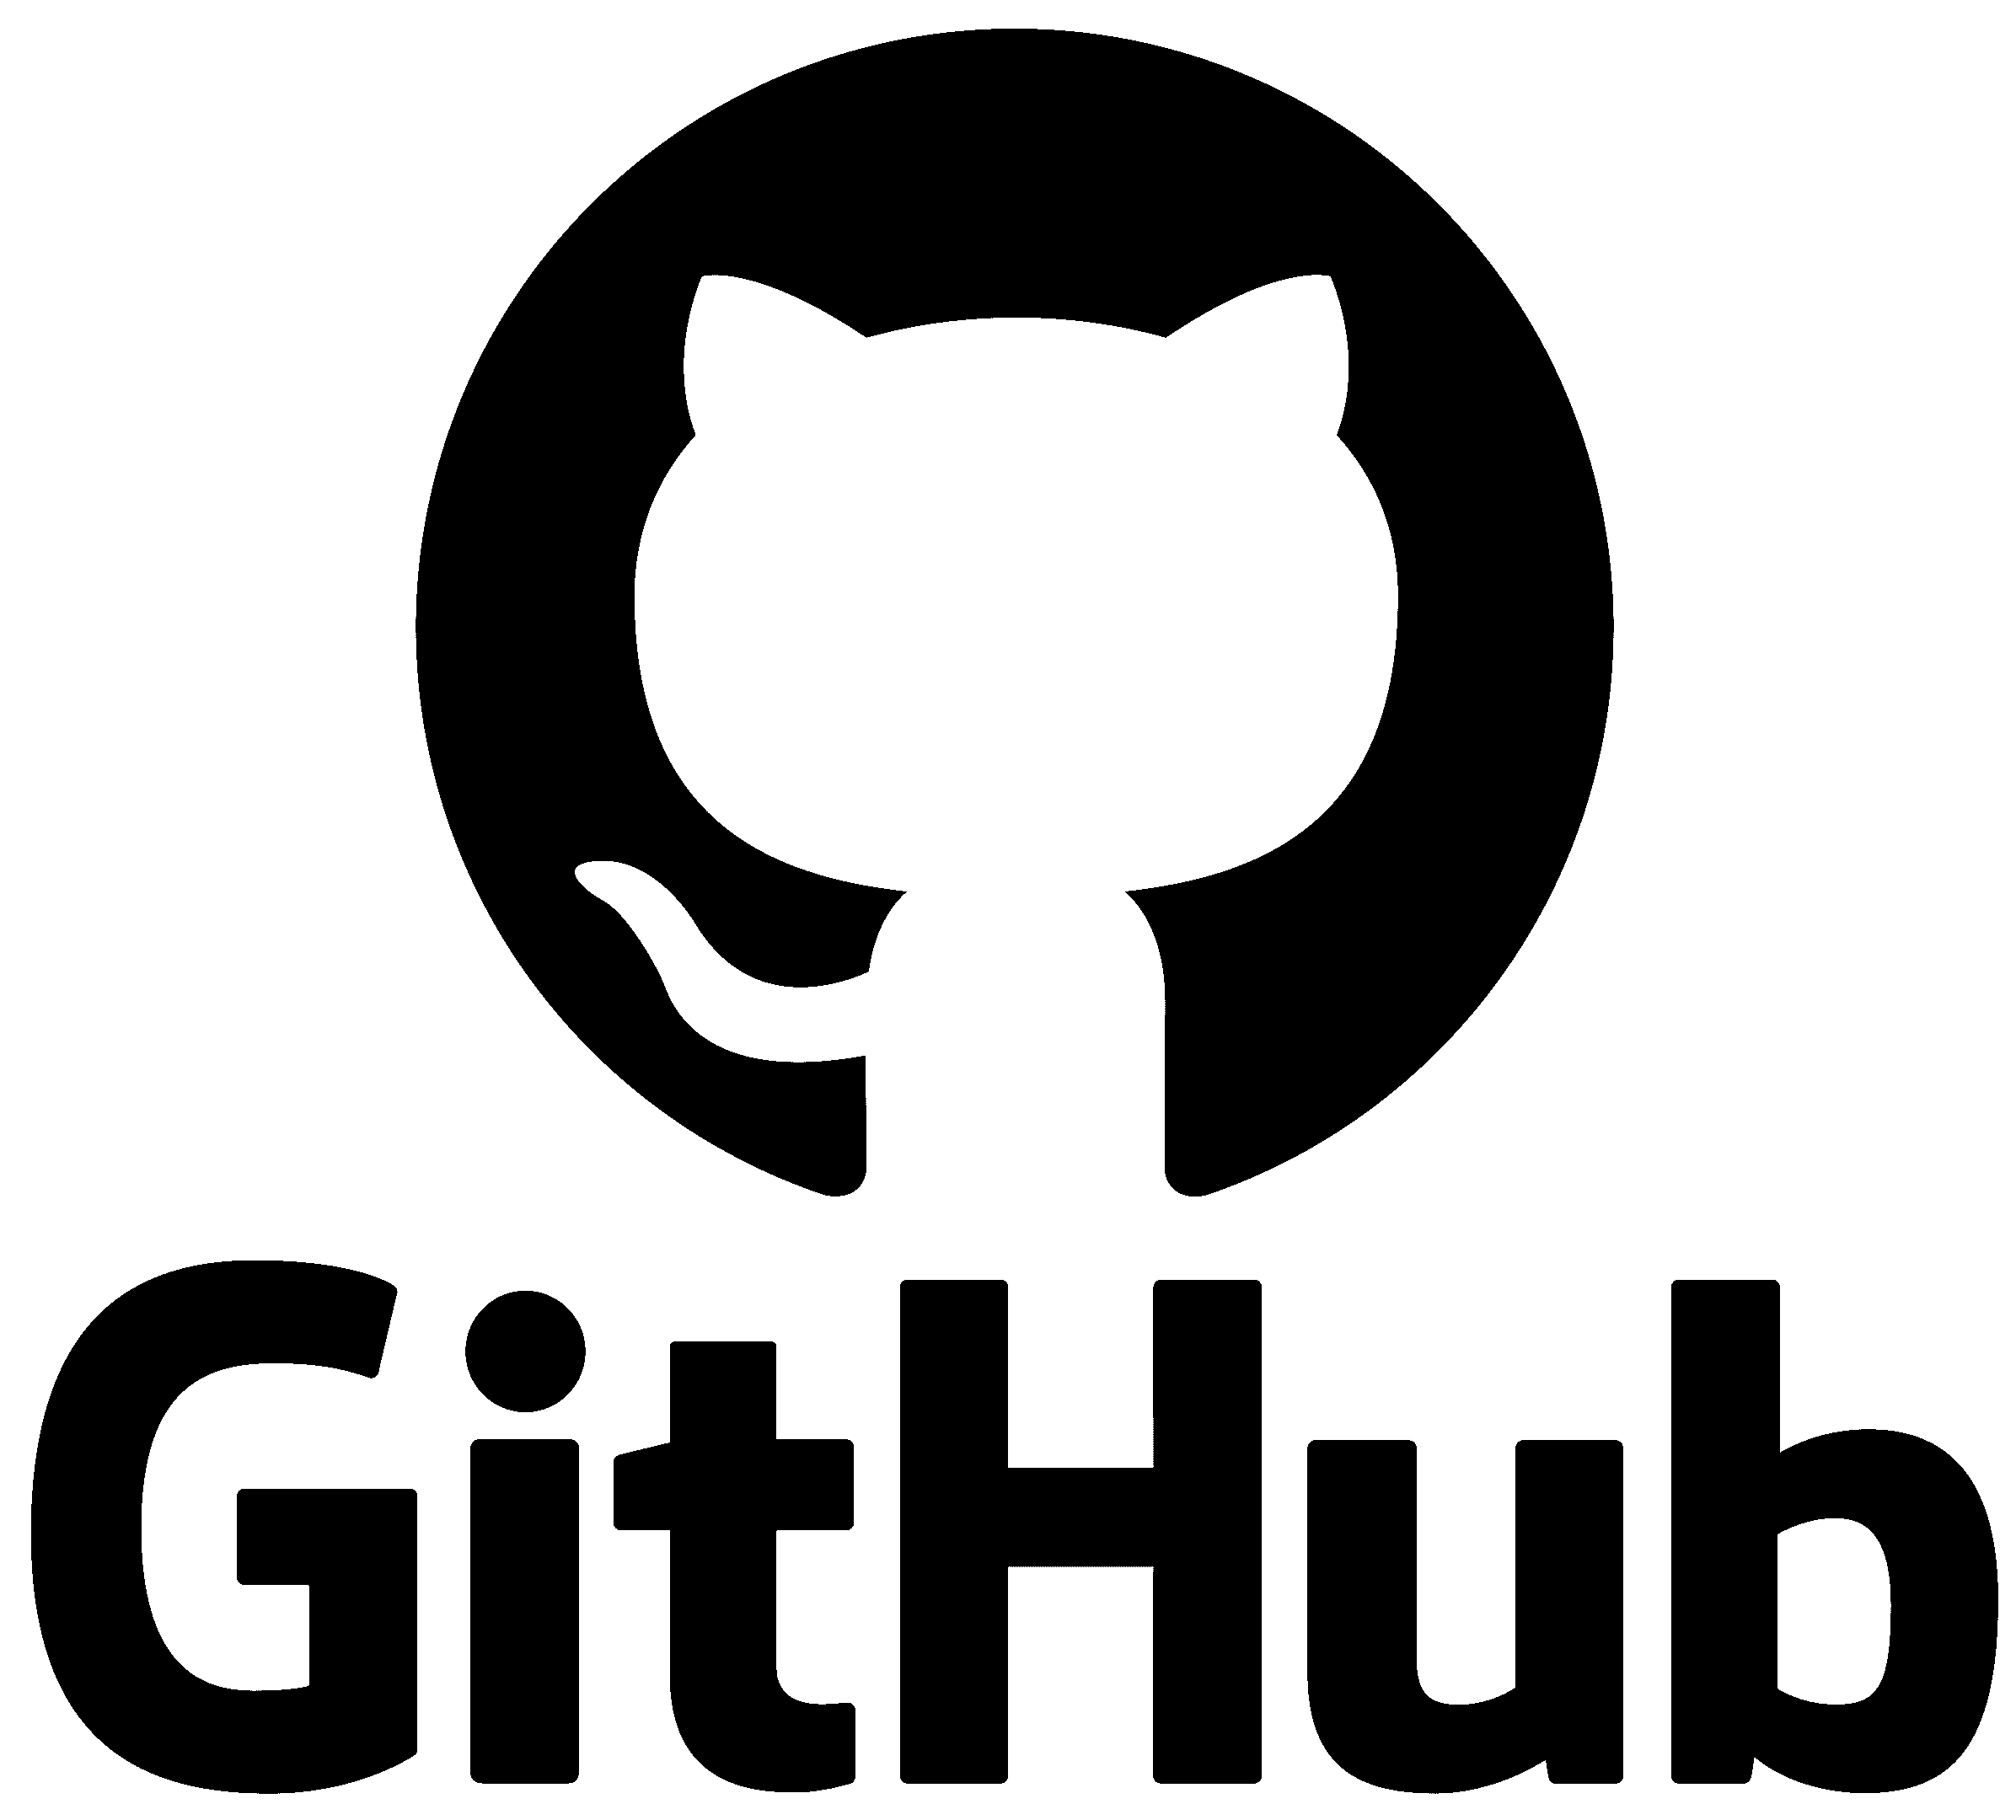
\includegraphics[width=0.7\textwidth]{gha-logo.png}
\end{minipage}
\vspace*{\fill}

%-------------------------------------------
\end{document}